\documentclass[11pt, a4paper]{article}

\usepackage[utf8]{inputenc}
\usepackage[a4paper, total={6in, 8in}]{geometry}
\raggedbottom

\usepackage{mlmodern}
\usepackage{csquotes}
\usepackage{parskip}
\usepackage[italian]{babel}
\usepackage{booktabs}
\usepackage{multicol}
\usepackage{graphicx}
\usepackage{fancyhdr}
\usepackage{float}
\usepackage{changepage}
\usepackage{fancyvrb}
\usepackage[final]{pdfpages}
\usepackage{placeins}
\usepackage{hyperref}
\usepackage[all]{hypcap}
\usepackage{tcolorbox}
\usepackage{xurl}
\usepackage{xcolor}
\usepackage{tikz}
\usepackage{biblatex}
\usepackage{array}
\usepackage{pdfpages}
\usepackage{multirow}
\usepackage{pgfplots}
\usepackage{listings}
\usepackage{caption}
\usepackage{pdfpages}
\usepackage{placeins}
\usepackage{graphicx}
\usepackage{tikz}
\usetikzlibrary{matrix}
\usepackage{colortbl}
\usepackage{ifthen}
\usepackage{listings}
\usepackage{mathtools}
\usepackage{subfig}
\usepackage{amsmath}
\DeclarePairedDelimiter\ceil{\lceil}{\rceil}
\DeclarePairedDelimiter\floor{\lfloor}{\rfloor}

\lstset{
	language=C++,
	tabsize=4,
	keepspaces,
	extendedchars=true,
	rulecolor=\color{black},
	basicstyle=\footnotesize,
	aboveskip=5pt,
	upquote=true,
	columns=fixed,
	showstringspaces=false,
	extendedchars=true,
	breaklines=false,
	frame=single,
	showtabs=false,
	showspaces=false,
	showstringspaces=false,
}

\usepgfplotslibrary{groupplots}
\pgfplotsset{compat=1.17}


\addbibresource{bibliography.bib}

\hypersetup{
	colorlinks=false,
	citecolor=black,
	filecolor=black,
	linkcolor=black,
	urlcolor=black,
	allbordercolors=white
}


\definecolor{codegreen}{rgb}{0,0.6,0}
\definecolor{codegray}{rgb}{0.5,0.5,0.5}
\definecolor{codepurple}{rgb}{0.58,0,0.82}
\definecolor{backcolour}{rgb}{0.95,0.95,0.92}

\lstdefinestyle{mystyle}{
	backgroundcolor=\color{backcolour},   
	commentstyle=\color{codegreen},
	numberstyle=\tiny\color{codegray},
	stringstyle=\color{codepurple},
	basicstyle=\ttfamily\footnotesize,
	breakatwhitespace=false,         
	breaklines=true,                 
	captionpos=b,                    
	keepspaces=true,                   
	numbersep=5pt,                  
	showspaces=false,                
	showstringspaces=false,
	showtabs=false,                  
	tabsize=1
}

\lstset{style=mystyle}

\setlength{\headheight}{14pt}

\begin{document}
	\begin{center}
	{\LARGE \textbf{Università degli Studi di Milano Bicocca}} \\
	\vspace{0.2cm}
	{\Large {Dipartimento di Informatica}} \\ 
	\vspace{1cm}
	
	
\includegraphics[width=4cm]{figures/unimib-logo.png} \\
	\vspace{0.4cm}
	
	{\huge \textbf{Metodi del calcolo scientifico}} \\ 
	\Large{Compressione di immagini attraverso la DCT}
	\vspace{3cm}
\end{center}
\vspace{2cm}

\noindent \large{Membri del gruppo:} 

\begin{tabular}{@{}lll}
	\textbf{Canesi Gabriele} & 851637 & \href{mailto:g.canesi1@campus.unimib.it}{\texttt{g.canesi1@campus.unimib.it}}\\
	\textbf{Fiorenza Gioele} & 851631 & \href{mailto:g.fiorenza1@campus.unimib.it}{\texttt{g.fiorenza1@campus.unimib.it}}\\
	\textbf{Ghislotti Gianluca} & 859242 & \href{mailto:g.ghislotti@campus.unimib.it}{\texttt{g.ghislotti@campus.unimib.it}}\\
\end{tabular}

\vfill
\begin{center}
	\large{\textbf{Anno Accademico 2022/2023}}
\end{center}




	\thispagestyle{empty}
	\newpage
	\pagestyle{fancy}
	\pagenumbering{roman}
	
	
	\tableofcontents
	
	\newpage
	
	\definecolor{fireenginered}{rgb}{0.81, 0.09, 0.13}
	\hypersetup{
		linkbordercolor=fireenginered
	}
	\pagenumbering{arabic}
	
		
\part{Implementazione della DCT2}

Lo scopo di questa parte del progetto è stato quello di implementare la nostra versione della DCT2 e confrontare i tempi di esecuzione con quelli di una libreria che implementa la versione fast della DCT2. La libreria utilizzata è la FFTW \cite{fftw}, scritta in C.

Per testare la scalatura eseguita da FFTW, applichiamo una dct e una idct su una matrice di partenza per poi testare se tali valori corrispondono tra loro. Dalla differenza dei risultati ottenuti, abbiamo osservato che viene introdotto un errore durante le operazioni non superiore ad 1e$^{-14}$. Consideriamo tale errore di approssimazione accettabile, osservando che la differenza tra 2 double successivi è pari a 2.22045e$^{-16}$.

L'implementazione "fatta in casa" della DCT2 e dell'analoga IDCT2 è stata implementata tramite la sua versione ad una singola dimensione, infatti una 2-D discrete cosine transform è semplicemente una doppia applicazione della versione ad una dimensione. Così facendo, abbiamo codificato la cosine transform ad una singola dimensione, per poi chiamarla sia sulle righe che sulle colonne, ottenendo in questo modo una 2-D cosine transform.

\section{Informazioni sulla libreria}

La libreria scelta, come accennato precedentemente, è la FFTw, il cui nome è l'abbreviativo di \textit{Fast Fourier Transform in the West}. Infatti si dichiara essere una delle implementazioni più veloci della Fastest Fourier Transform. Tali risultati sono stati raggiunti grazie ad un ottimizzazione particolare degli algoritmi, che sfruttano alcune istruzioni specifiche dei vari processori ottimizzate per la risoluzione numerica.

L'implementazione effettiva risale al '97, nonostante ciò gode di particolare popolarità su Github\cite{Github} e ha vinto numerosi premi, tra cui il \textit{1999 J.H Wilkinson Prize for Numerical Software}, il quale viene conferito, una volta sola ogni 4 anni, al software che "best addresses all phases of the preparation of high quality numerical software", ovvero al programma che meglio copre tutte le fasi di un software numerico. Inoltre il paper correlato alla libreria "A Fast Fourier Transform Compiler"\cite{fftw_paper} ha ricevuto il premio di "Most Influential PLDI Paper" nel 2009, con un totale di circa 2000 download e 400 citazioni.

\section{Implementazione custom}

Il codice implementato per eseguire la DCT, secondo la definizione de coefficienti vista a lezione, è il seguente:


\begin{lstlisting}[gobble=1]
	void dct(int N, double *in, double *out, int jump = 1) {
		
		double *f = new double[N];
		
		for (int i = 0; i < N; ++i) {
			f[i] = in[i * jump];
		}
		
		for (int i = 0; i < N; ++i) {
			
			double a_i = 0;
			
			for (int j = 0; j < N; ++j) {
				a_i +=  f[j] * cos(i * M_PI * (2 * j + 1) / (2 * N));
			}
			
			a_i /= (i == 0 ? N : N/2);
			out[i * jump] = a_i;
		}
		
		delete[] f;
	}

\end{lstlisting}

Siccome l'applicazione di 2 dct genera la DCT2, di seguito si trova la sua implementazione:

\begin{lstlisting}[gobble=1]
	void dct2(int N, int M, double *in, double *out) {
		for (int i = 0; i < N * M; ++i) {
			out[i] = 0;
		}
		
		// Rows
		for (int i = 0; i < N; ++i) {
			dct(M, in + i * M, out + i * M, 1);
		}
		
		// Columns
		for (int i = 0; i < M; ++i) {
			dct(N, out + i, out + i, M);
		}
	}
\end{lstlisting}

Il codice della DCT prende in input il puntatore alla matrice di output per fare in modo che la DCT2 possa eseguire due DCT in place, ovvero scrivendo due volte sulla stessa matrice evitando ulteriori allocazioni di memoria.

Per evitare il calcolo del prodotto scalare delle basi con sè stesse, inoltre, abbiamo controllato direttamente l'indice della frequenza: se questo è 0, allora il prodotto scalare sarà N, altrimenti corrisponderà sempre a $\frac{N}{2}$.

Inoltre, è presente un parametro \textit{jump}, che fa in modo che la DCT salti di un certo numero di celle di memoria per passare da una componente alla successiva: la sua utilità si concretizza nel momento in cui viene chiamata la DCT sulle colonne: la matrice è organizzata in modalità row major, per cui, per eseguire la dct in place sulle colonne, è necessario dire alla DCT di saltare di M celle per passare alla componente successiva del vettore "logico", dove M rappresenta il numero di colonne della matrice.

\section{Test}

All'interno del codice sono stati aggiunti una serie di test (tramite l'uso delle assert) all'interno dei quali viene verificato l'esito dell'applicazione della DCT e della IDCT sulla matrice e sul vettore fornito. Successivamente l'esecuzione del codice prosegue verificando i tempi e generando un csv contenente i risultati delle esecuzioni su matrici man mano sempre più grandi. Dai risultati presenti nell'immagine \ref{fig:timings}, si può osservare come l'implementazione "fatta in casa" (in figura denominata \textit{Slow}) abbia effettivamente un andamento più esponenziale rispetto la liberia (in figura \textit{Fast}). Un fenomeno particolare che si osserva è che mentre la matrice è ancora di dimensioni molto ristrette la dct implementata fatta da noi supera quella fast. Una possibile ragione è che la FFTW utilizza delle tecniche numeriche sulla trasformata per ridurre il numero di operazioni necessarie, il che porta ad una maggiore efficienza per matrici di elevate dimensioni. Analogamente, nelle matrici di piccole dimensioni, è ragionevole pensare che l'applicazione di queste tecniche introducano un overhead che porta ad avere una performance peggiore rispetto alla DCT2 standard.

FFTW non esegue lo stesso algoritmo ad ogni chiamata della DCT: questo è il motivo per cui il grafico della versione fast non è liscio come quello della versione "fatta in casa", che esegue sempre lo stesso tipo di istruzioni indipendentemente dalla matrice/vettore in input.
È importante puntualizzare inoltre che, anche se questo non influisce sui tempi, i risultati delle DCT e DCT2 sono diversi tra la versione fast e la nostra: infatti, la libreria presa in considerazione utilizza un tipo di scaling della matrice dei coefficienti diverso da quello visto a lezione.

\begin{figure}[ht]
	\centering
	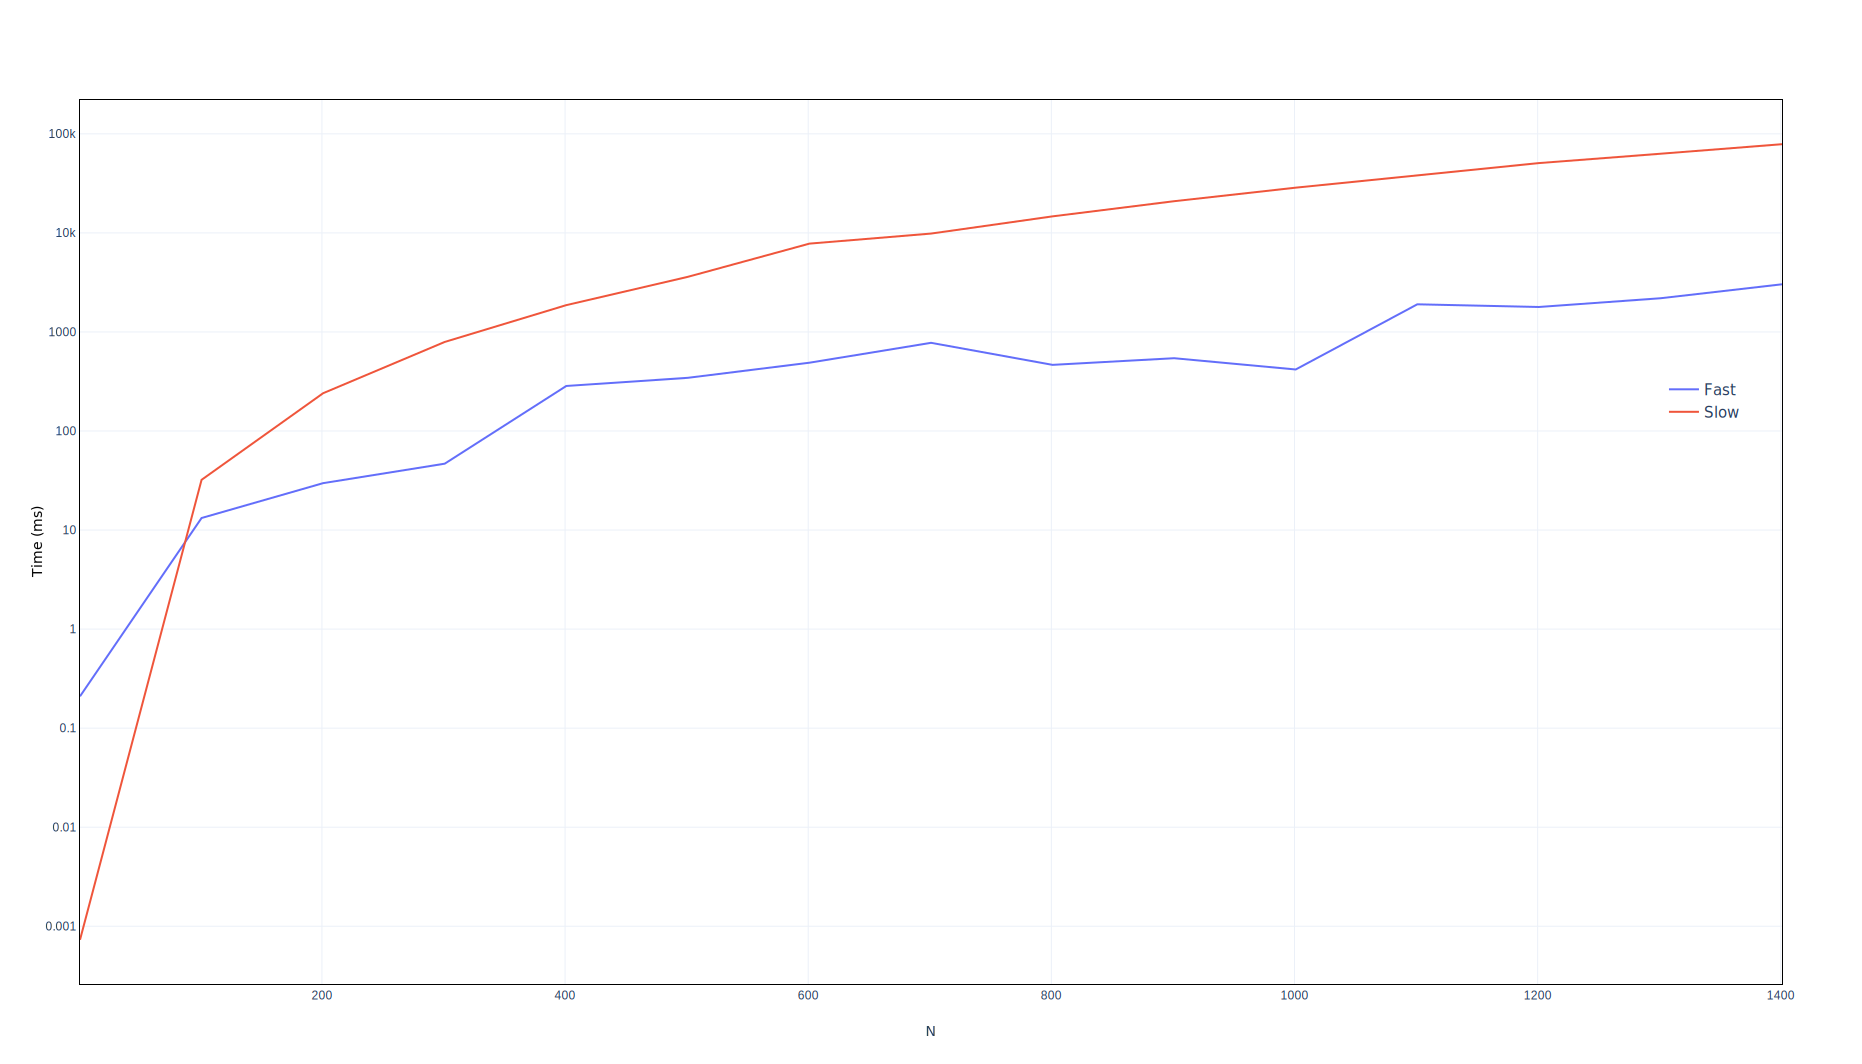
\includegraphics[scale=0.7]{figures/timings}
	\caption{Tempi}
	\label{fig:timings}	
\end{figure}

\FloatBarrier
	\part{Progettazione di un'interfaccia grafica per la compressione di immagini}

L'interfaccia grafica è realizzata con l'ambiente di sviluppo Qt\cite{qt}, il quale permette di creare delle GUI scrivendo il codice in linguaggio C++. La compressione applicata è stata limitata solamente alla visualizzazione, ovvero l'immagine perde l'informazione legata alle alte frequenze, però le strutture dati che contengono tale immagine rimangono costanti. Introducendo la possibilità, ad un successivo salvataggio dell'immagine, di memorizzare solamente i coefficienti diversi da 0, richiamando un concetto di simil sparsità però applicato alle frequenze non tagliate dalla compressione.

Il programma fornisce una schermata nella quale è possibile selezionare l'immagine da comprimere e i valori di compressione da applicare, ossia dimensione dei blocchi e la soglia di taglio delle frequenze. Nella parte sinistra della GUI viene mostrata l'immagine originale, mentre in quella di destra la sua versione compressa. In figura\ref{fig:deer} è riportato un esempio sull'immagine \textit{deer}, sulla quale sono stati applicati blocchi di elevate dimensioni (70x70) ed una elevata compressione (circa del 92\%), in questo modo è facilmente osservabile l'effetto della compressione sui blocchi e sull'immagine.

\begin{figure}[h]
	\centering
	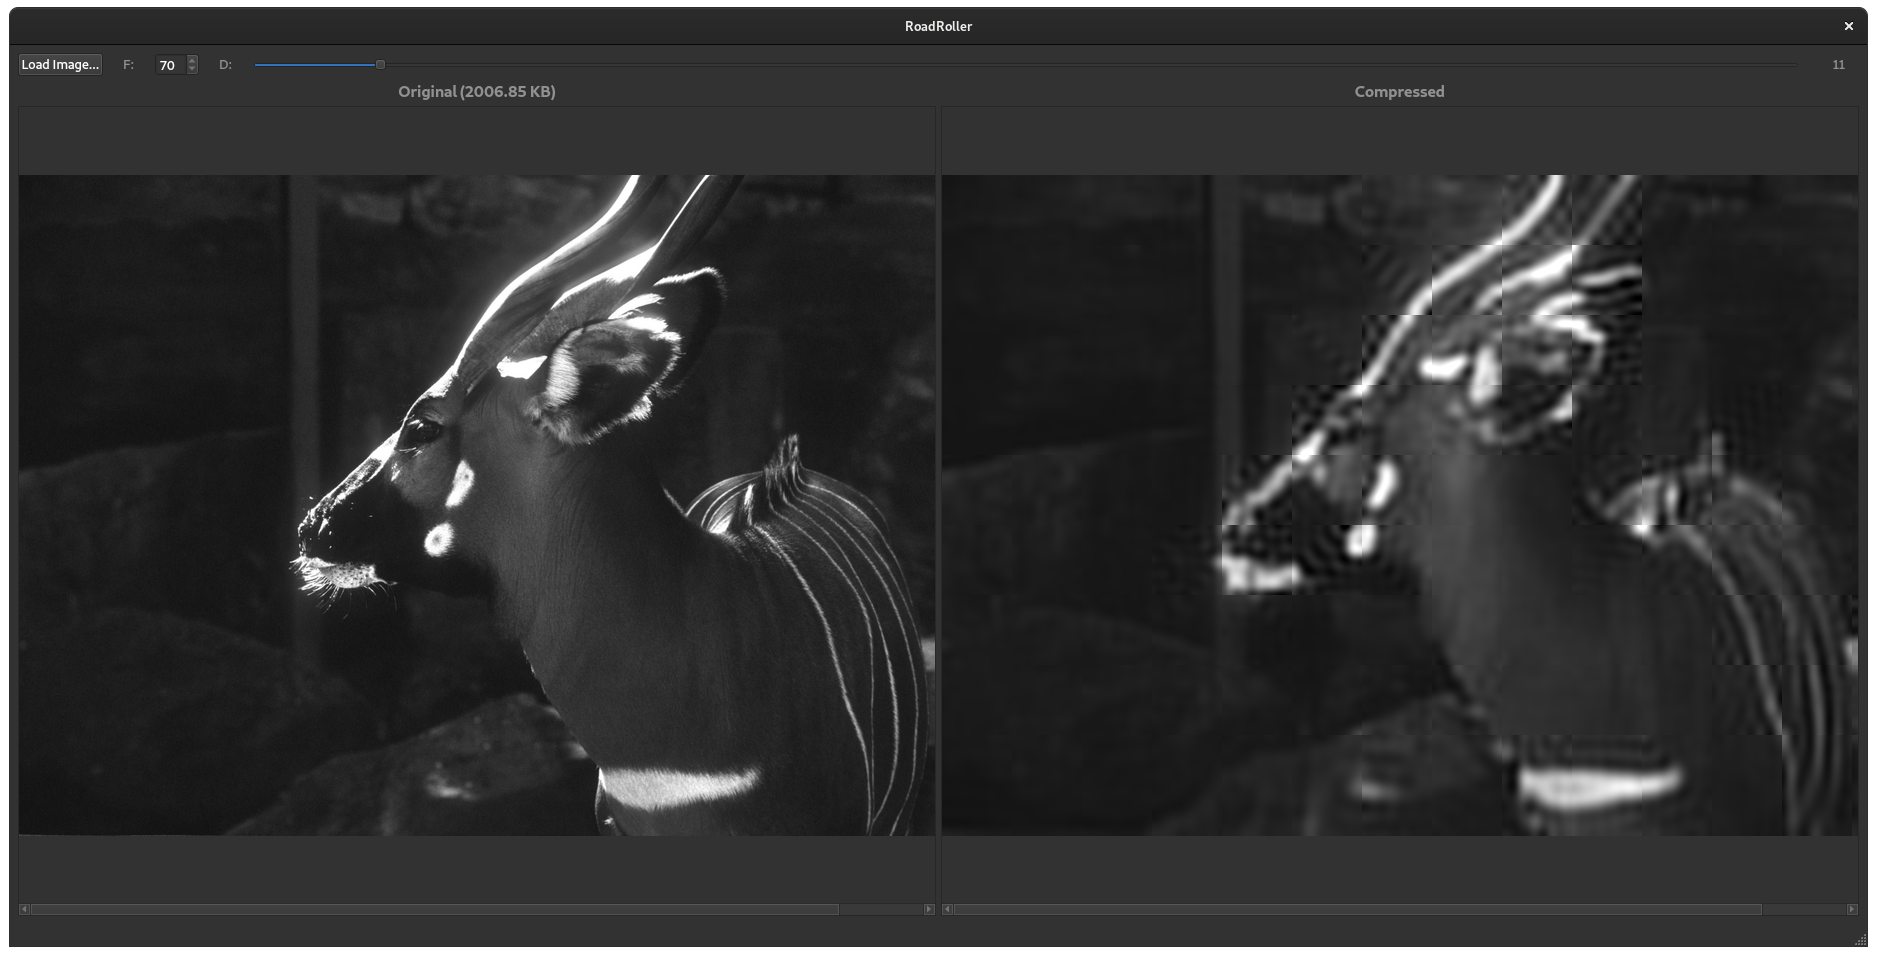
\includegraphics[width=1\linewidth]{figures/qt_deer}
	\caption{Programma di compressione basato su Qt}
	\label{fig:deer}
\end{figure}

\section{Features}

Alla versione base del progetto, descritto precedentemente, sono state aggiunte un insieme di funzionalità:

\begin{itemize}
	\item \textbf{Multithreading}: L'aggiunta dei thread permette una rapida compressione dell'immagine. Infatti essendo che i blocchi lavorano su aree della figura indipendenti gli uni dagli altri, è possibile eseguire le compressioni in parallelo, così come la scrittura dei pixel nell'oggetto immagine finale.
	
	Abbiamo fatto in modo che i blocchi vengano suddivisi in una griglia la cui quantità di celle di celle corrisponde al numero di core del sistema. In questo modo, il carico di lavoro può essere distribuito in modo equo tra i processori e minimizzare il tempo di esecuzione della compressione.
	\item \textbf{Navigazione dell'immagine}: All'interno dell'interfaccia grafica sono presenti degli slider e dei tasti per zoomare nelle immagine, tali tasti sono sincronizzati in modo tale da poter visionare contemporaneamente le stesse zone delle 2 immagini. In questo modo si possono osservare più comodamente i vari effetti che la compressione comporta sulle immagini.
	\item \textbf{Aggiornamento in tempo reale}: Grazie ai thread, che velocizzano notevolmente il lavoro, modificando la dimensioni dei blocchi e/o la dimensione del taglio delle frequenze, é possibile visionare nella parte di destra gli aggiornamenti sulla compressione, in tempo reale. Il delay che intercorre tra la modifica del parametro e il suo aggiornamento é solitamente molto basso, anche se ovviamente varia in relazione alla dimensione dell'immagine passata in input.
	\item  \textbf{Gestione dei bordi}:  A fini sperimentali, abbiamo provato ad implementare il processo di compressione in modo che venga effettuata la dct anche su blocchi più piccoli sui bordi dell'immagine, in modo da ricoprirne l'intera superficie.
\end{itemize}

\section{Gestione dei pixel in eccesso}

All'interno di questo progetto, abbiamo deciso in modo "sperimentale" di gestire in maniera leggermente diversa da jpeg i pixel sui margini.

Nello specifico, il nostro programma di compressione crea dei piccoli blocchi in modo da riempire completamente tutta l'immagine e ne esegue la DCT2. Prima di eseguire il taglio, però, il valore del taglio viene adattato in modo da essere proporzionato alla minore quantità di frequenze e da rendere, quindi, la compressione dell'immagine più uniforme:

$$d' = d  \sqrt{ \frac{W \cdot H}{F^{2}}}$$

dove W e H rappresentano rispettivamente la larghezza e l'altezza del blocco preso in considerazione.
Inoltre, nel caso in cui $d'=0$, ma $d>0$, si mantiene il valore originale al fine di evitare buchi indesiderati.

Abbiamo preso questa decisione perché, a differenza di jpeg, non siamo stati vincolati dalla matrice di quantizzazione e abbiamo potuto, quindi, sperimentare una gestione leggermente diversa del margine dell'immagine.


\begin{figure}
	\begin{minipage}{0.5\textwidth}
		\begin{center}
		
			\begin{tikzpicture}
				[%%%%%%%%%%%%%%%%%%%%%%%%%%%%%%
				box/.style={rectangle,draw=black,thick, minimum size=1cm},
				]%%%%%%%%%%%%%%%%%%%%%%%%%%%%%%
				
				\foreach \x in {0,1,...,3}{
					\foreach \y in {0,1,...,3}
					\node[box, fill=red] at (\x,\y){};
				}
			
			
				\foreach \x in {0,...,3}{
					\foreach \y in {0,...,3} {
						\ifnumcomp{\x + (3 - \y)}{<}{5}{
							\node[box, fill=green] at (\x,\y){};
						}{};
					}
				}
				
				
			\end{tikzpicture}
		\end{center}
		\begin{center}
			(a)
		\end{center}
	\end{minipage}\hfill
	\begin{minipage}{0.5\textwidth}
		\begin{center}
			\begin{tikzpicture}
				[%%%%%%%%%%%%%%%%%%%%%%%%%%%%%%
				box/.style={rectangle,draw=black,thick, minimum size=1cm},
				]%%%%%%%%%%%%%%%%%%%%%%%%%%%%%%
				
				\foreach \x in {0,1,...,2}{
					\foreach \y in {0,1,...,3}
					\node[box, fill=red] at (\x,\y){};
				}
				
				
				\foreach \x in {0,...,2}{
					\foreach \y in {0,...,3} {
						\ifnumcomp{\x + (3 - \y)}{<}{5}{
							\node[box, fill=green] at (\x,\y){};
						}{};
					}
				}
				
				
			\end{tikzpicture}
		\end{center}
	\begin{center}
		(b)
	\end{center}
\end{minipage}
\caption{Taglio delle frequenze sulle diverse dimensioni dei blocchi}\label{fig:taglio}
\end{figure}

\section{Visualizzazione dei risultati}

Per mostrare meglio la compressione potremmo momentaneamente ignorare la conversione dei valori tramite la IDCT2. In figura\ref{fig:compression_values} viene mostrato il risultato ottenuto, dove è possibile osservare i coefficienti generati dalla DCT, i quali vengono successivamente tagliati per il valore di input scelto. In questo modo, ogni blocco conterrà dati diversi da 0 solo nella parte superiore del taglio, evidenziata anche graficamente dalla distribuzione del colore bianco nei singoli blocchi. Infatti tale tonalità rappresenta un valore elevato del coefficiente presente nella matrice, mentre le zone nere, rappresentano i valori che sono stati impostati a 0 dal taglio.

\begin{figure}[h]
	\centering
	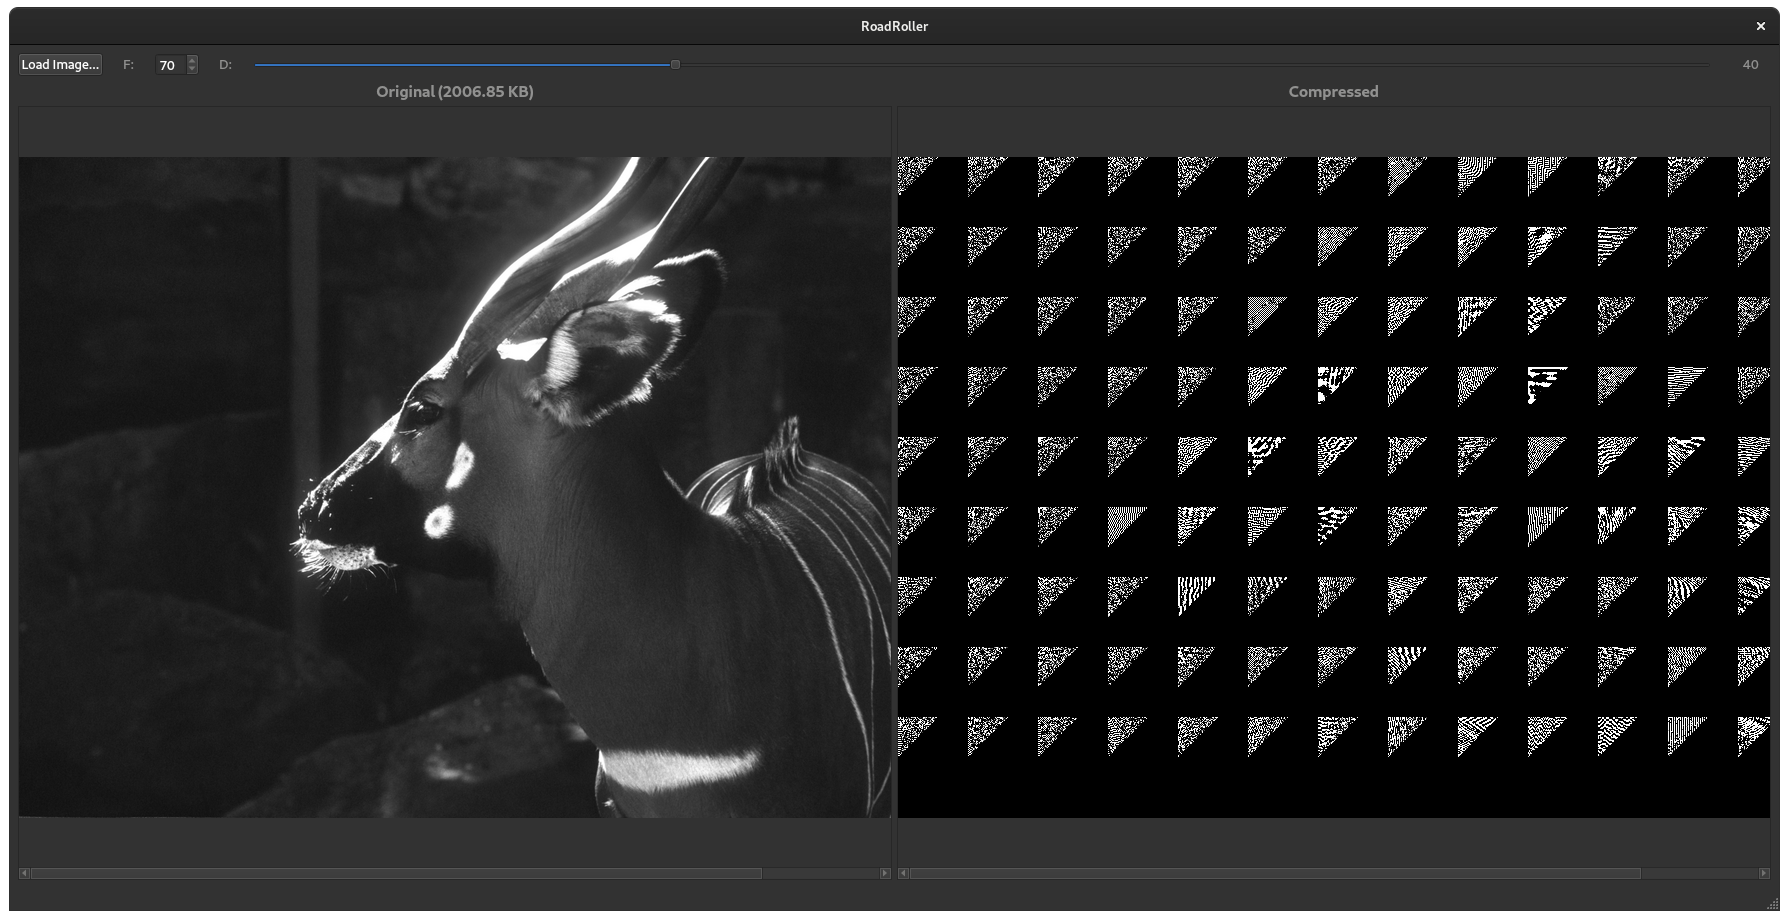
\includegraphics[width=1\linewidth]{figures/qt_dct_values}
	\caption{Valori della DCT generati dalla compressione (a meno dello scaling)}
	\label{fig:compression_values}
\end{figure}

\subsection{Fenomeno di Gibbs}

Scegliendo un'elevata dimensione dei blocchi si ottiene comunque il fenomeno di Gibbs, visibile chiaramente in Figura \ref{fig:gibbs}. Dove l'elevato contrasto tra il muso del cervo e il relativo sfondo, generano un repentino cambio di colore, il quale comporta l'apparizione degli artefatti sotto forma di onde nell'immagine finale.

Per rappresentare meglio il fenomeno, nel grafico di Figura \ref{fig:dct_values_on_gibbs} sono stati rappresentati i coefficienti della DCT relativi al blocco precedentemente illustrato, che presenta tale fenomeno. Per una migliore visualizzazione, la scala è stata ristretta, in questo modo non è possibile osservare la totalità del peso delle basse frequenze, ma in compenso si osserva meglio la distribuzione dei coefficienti su tutte le restanti frequenze.

Nell'istogramma le basse frequenze hanno valori nell'ordine di \path{1e+6}, mentre allontanandosi troviamo coefficienti che sono in proporzione molto più piccoli (nell'ordine delle migliaia), visibili in Figura \ref{fig:last_dct_values_gibbs}. Tali valori però sono fondamentali nella corretta rappresentazione dell'immagine, infatti essi riescono a modellare il repentino cambio di colore presente nel blocco analizzato. Quindi nel momento in cui essi vengono tagliati dalla compressione, si ottiene il fenomeno illustrato precedentemente in Figura \ref{fig:gibbs}

\begin{figure}[h]
	\centering
	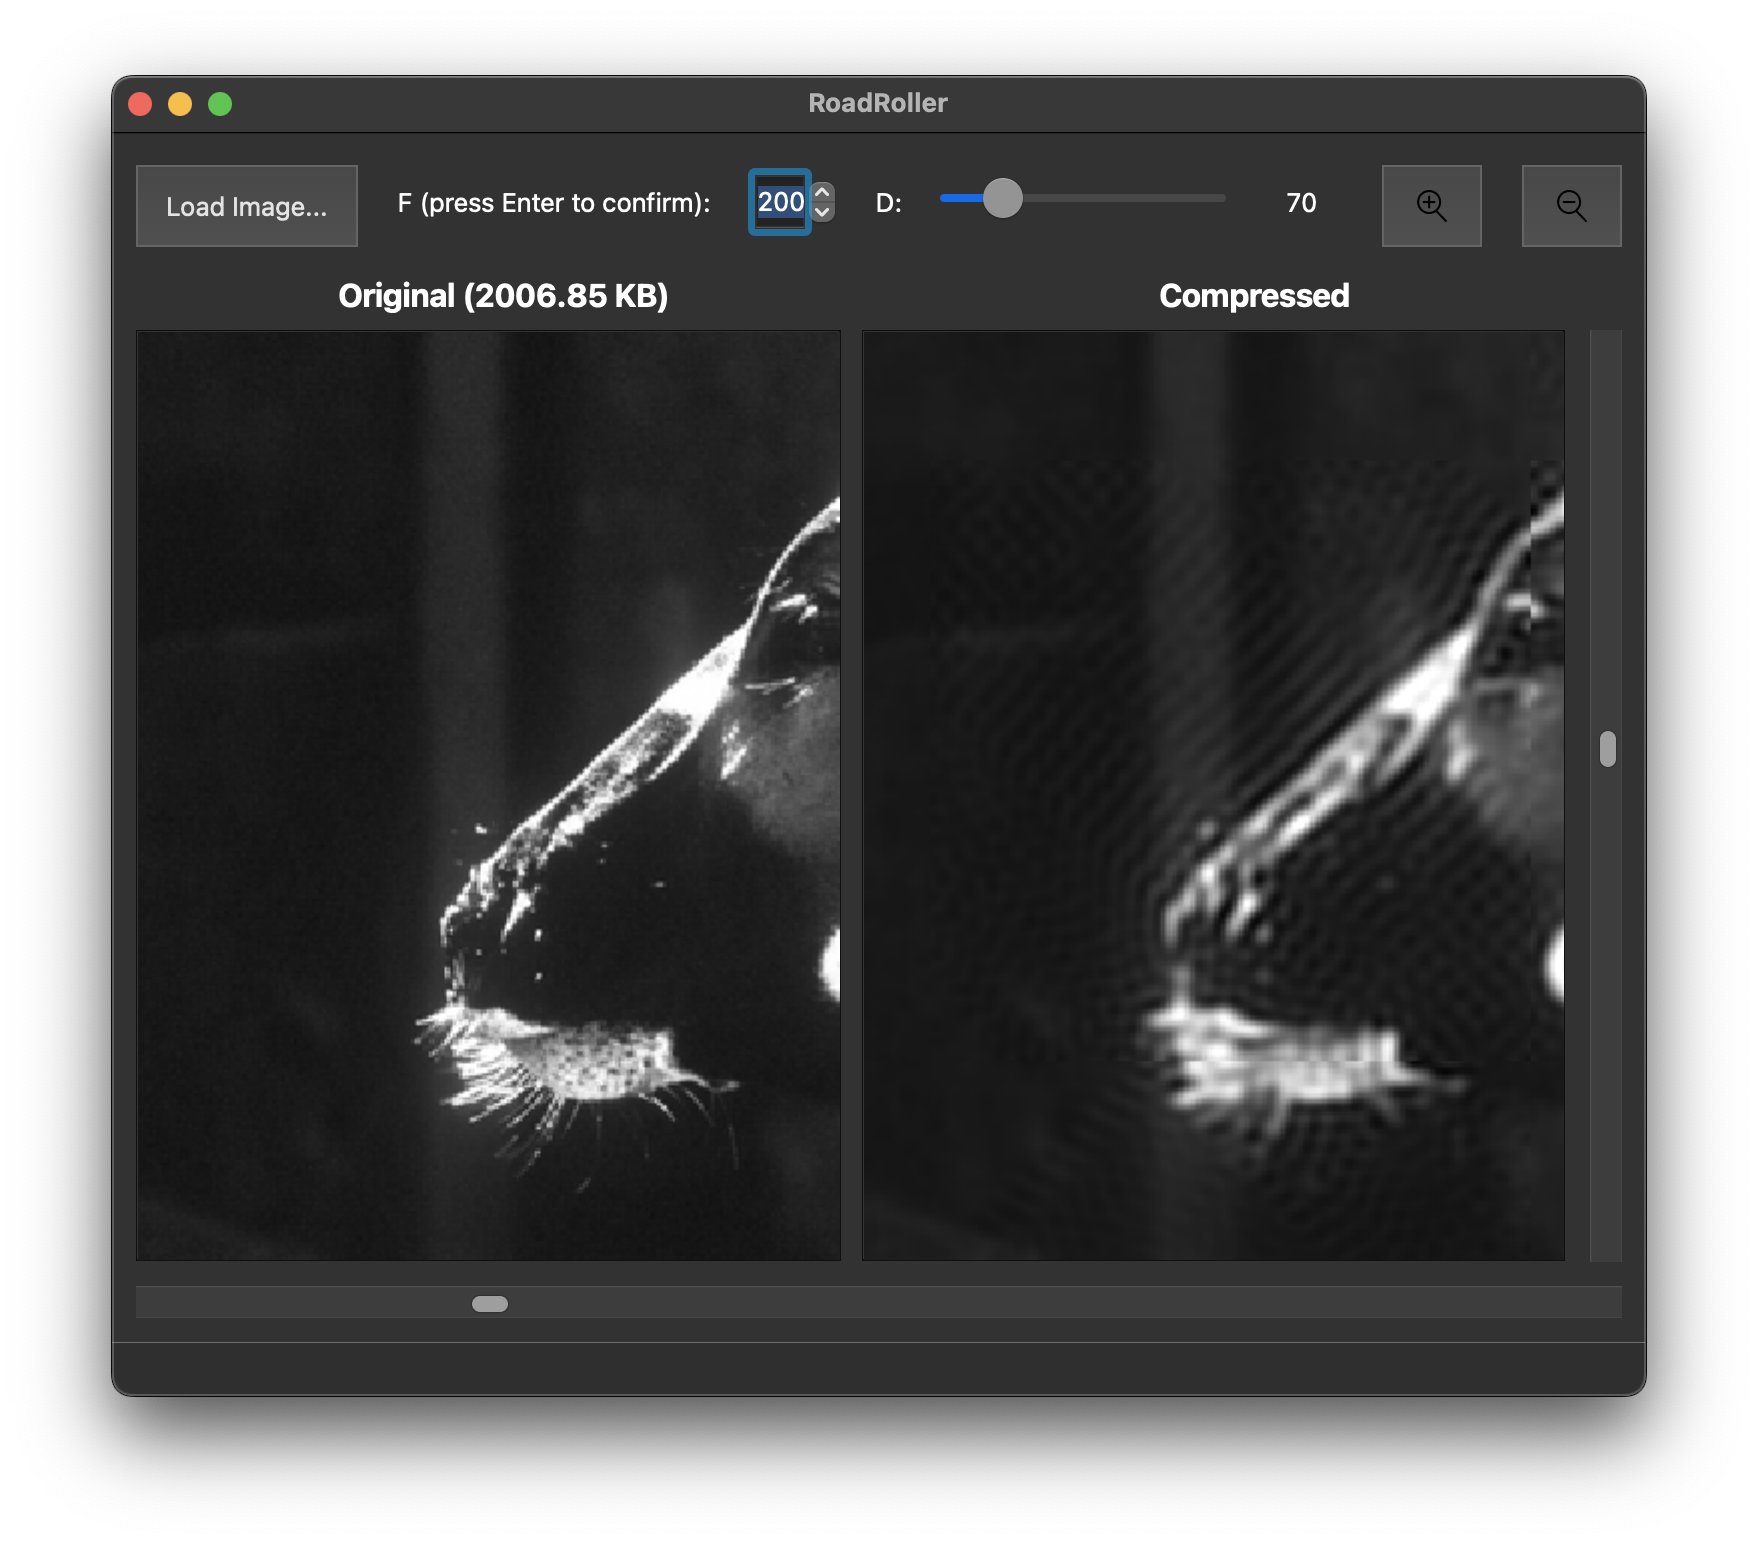
\includegraphics[width=1\linewidth]{figures/gibbs_phenomenon}
	\caption{Fenomeno di Gibbs su un blocco}
	\label{fig:gibbs}
\end{figure}


\begin{figure}
	\centering
	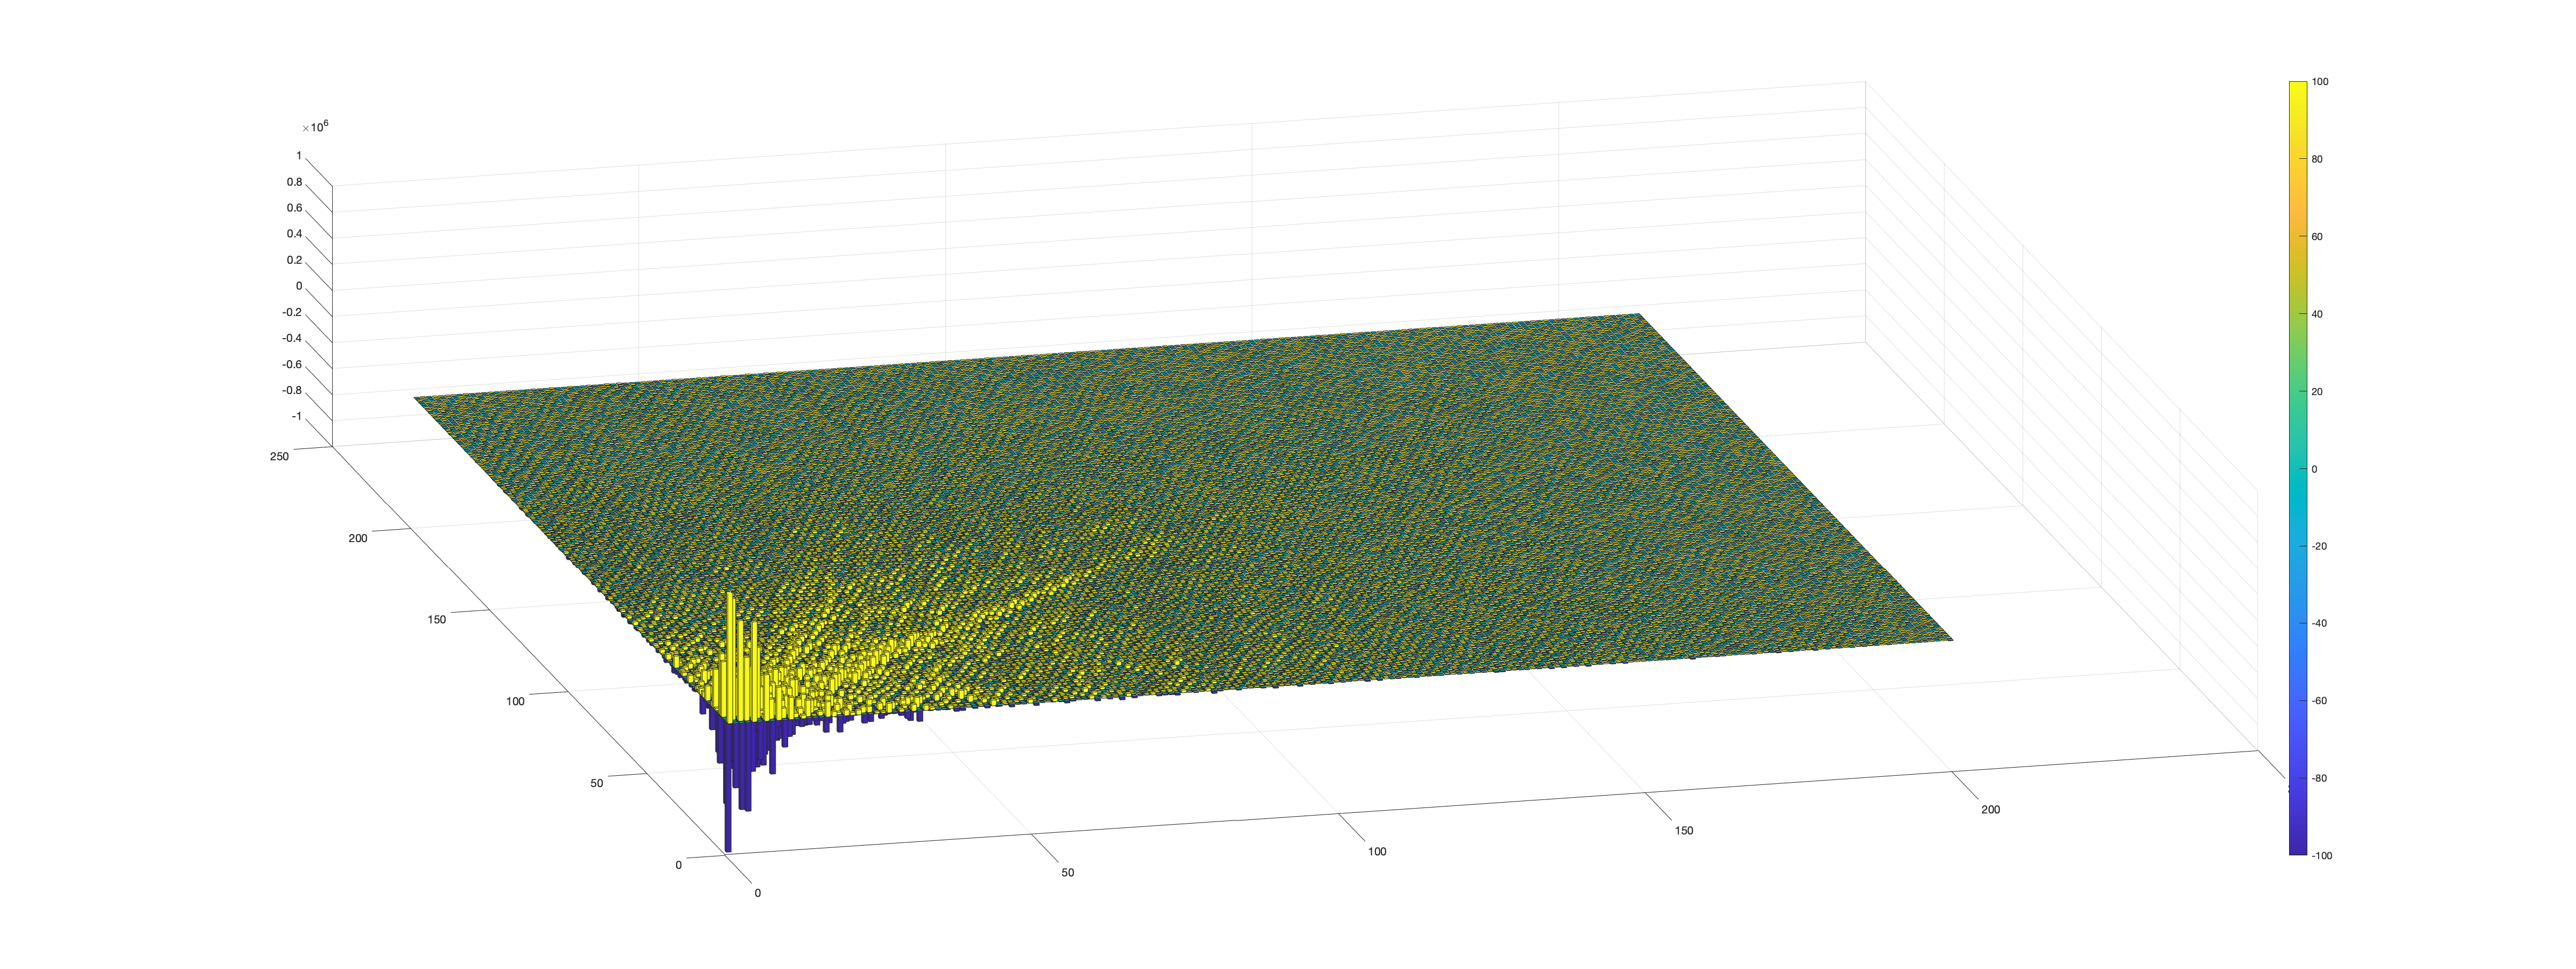
\includegraphics[width=1\linewidth]{figures/dct_values_3d.eps}
	\caption{Coefficienti DCT nel blocco mostrato in Figura \ref{fig:gibbs}}
	\label{fig:dct_values_on_gibbs}
\end{figure}

\begin{figure}
	\centering
	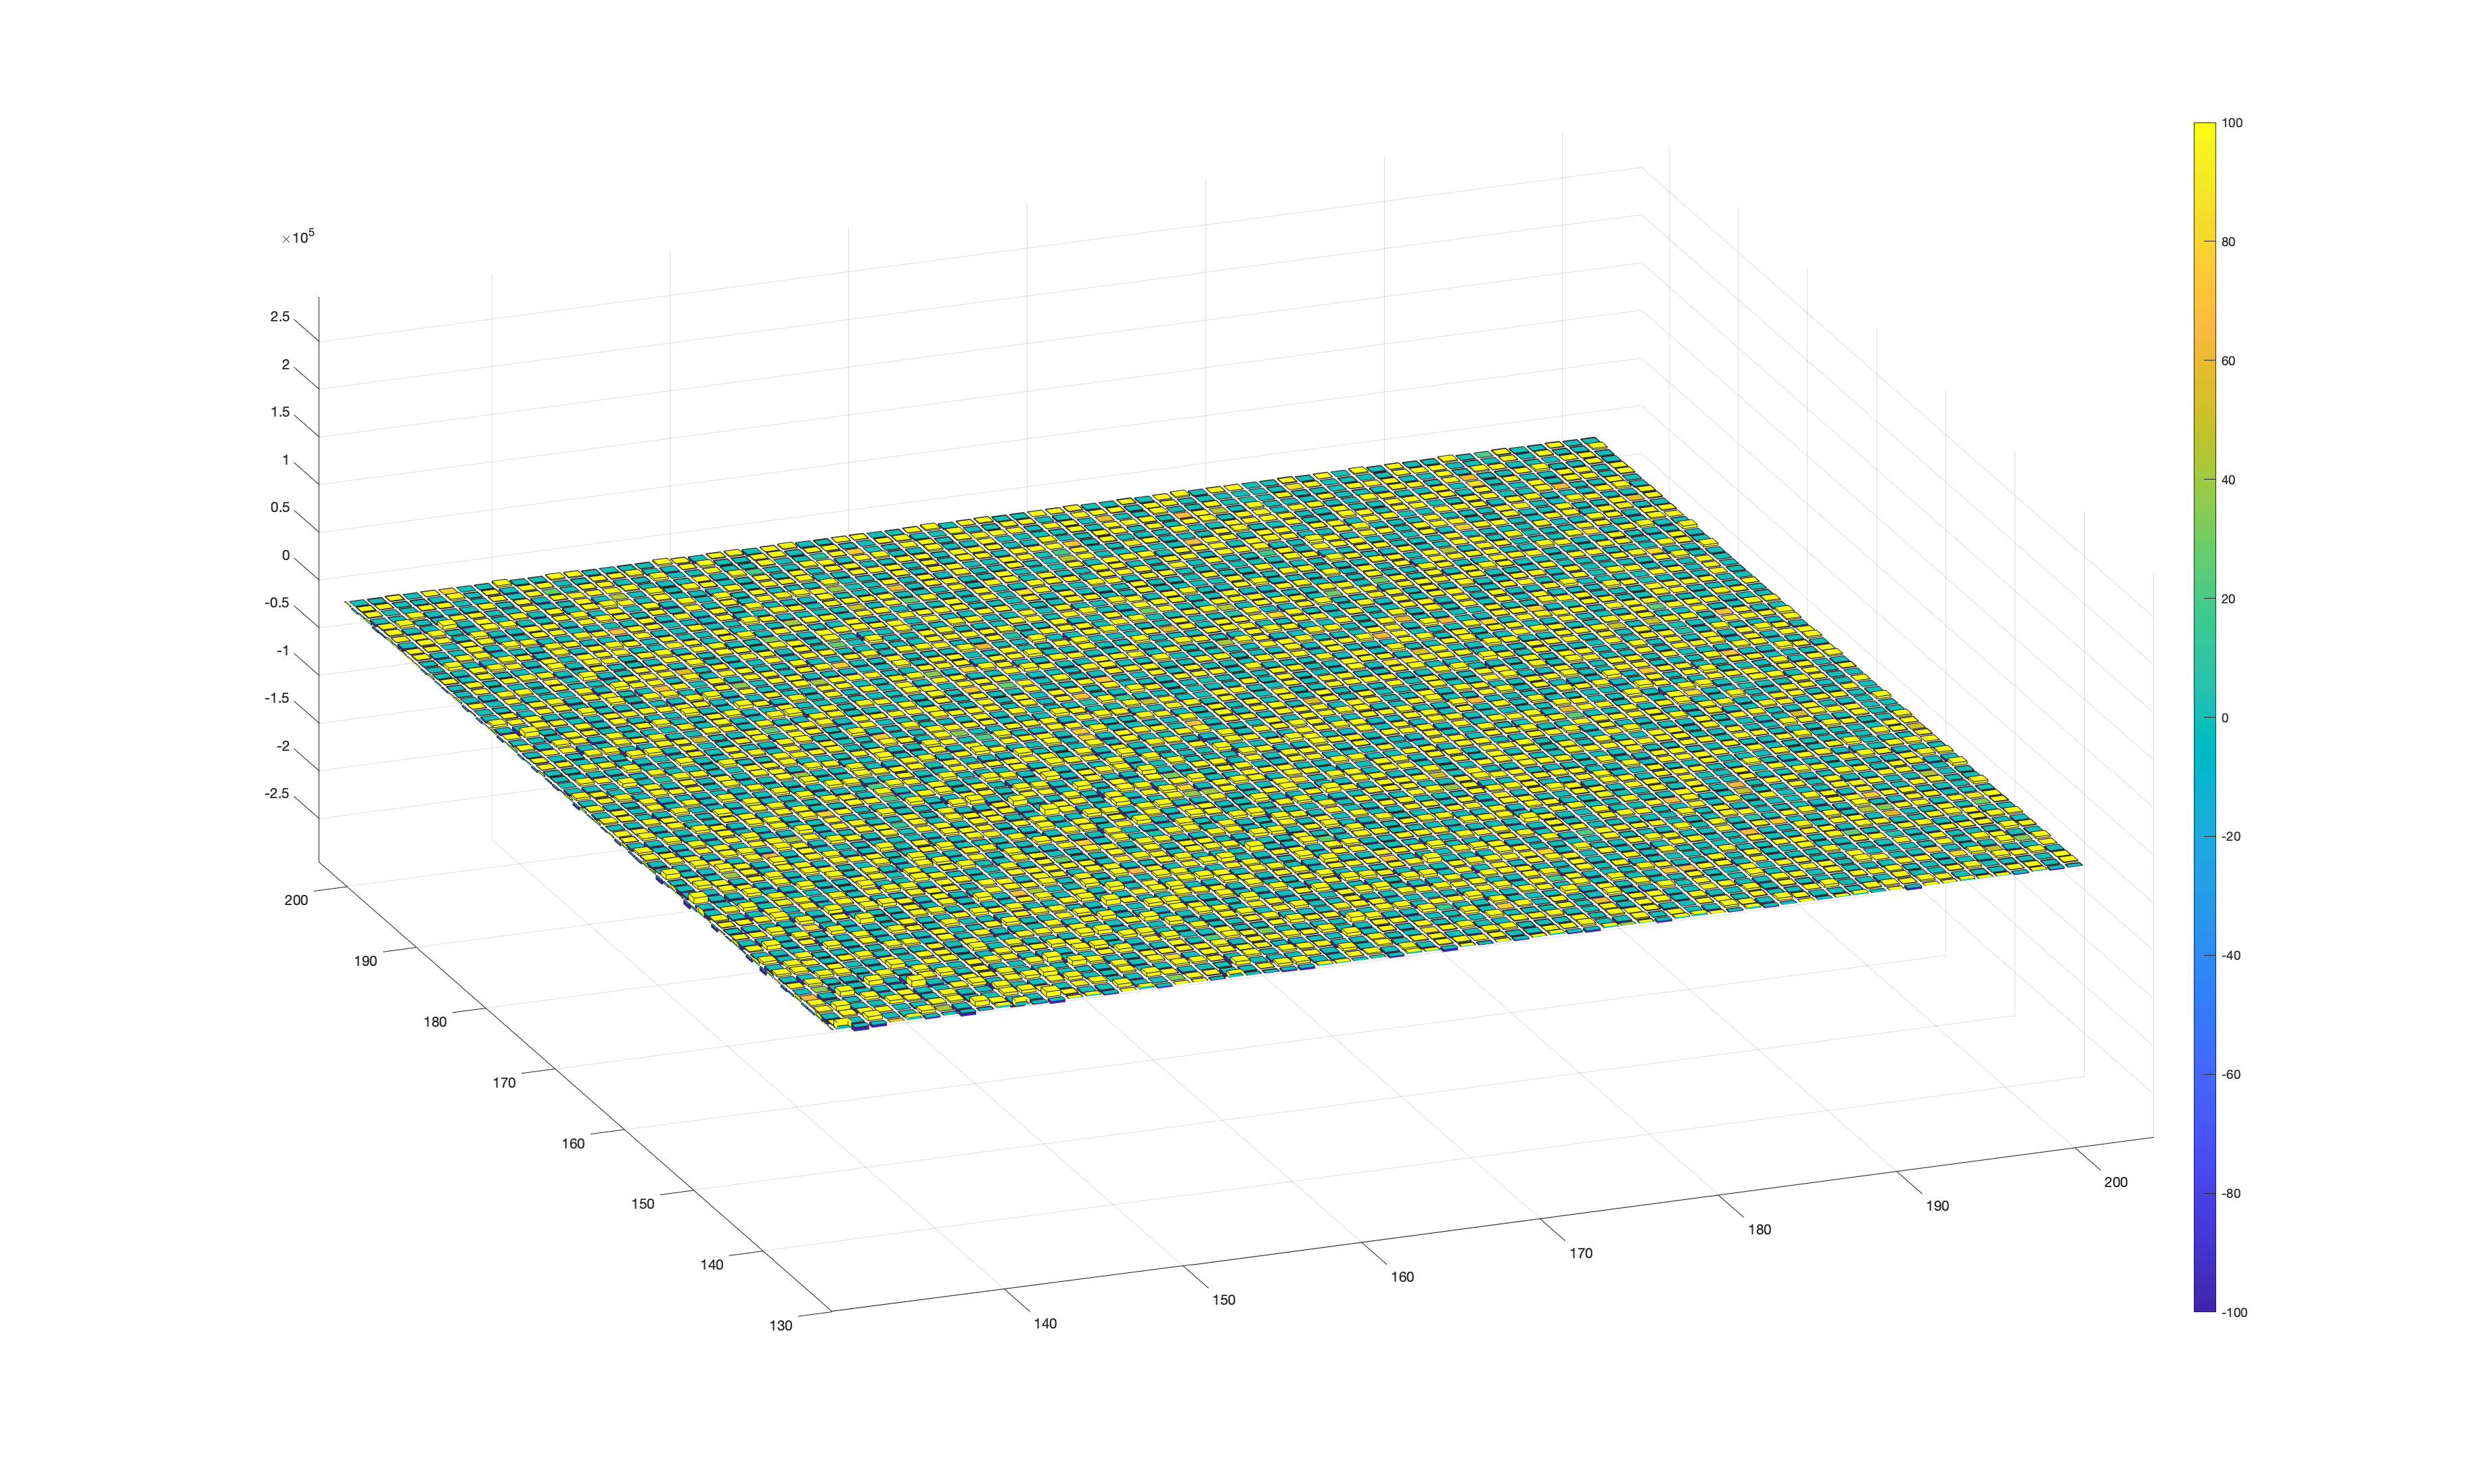
\includegraphics[width=1\linewidth]{figures/last_dct_values.eps}

	\caption{Ultimi 50 x 50 coefficienti della DCT relativi alla Figura \ref{fig:dct_values_on_gibbs}}
	\label{fig:last_dct_values_gibbs}
\end{figure}
	
	\FloatBarrier
	\newpage
	\printbibliography
\end{document}
	
